\documentclass{../tex/report}
\usepackage{setspace} % Setting line spacing
\usepackage{ulem} % Underline
\usepackage{caption} % Captioning figures
\usepackage{subcaption} % Subfigures
\usepackage{geometry} % Page layout
\usepackage{multicol} % Columned pages
\usepackage{multirow}
\usepackage{array,etoolbox}
\usepackage{fancyhdr}
\usepackage{enumitem}
\usepackage{tabularx}
\usepackage[toc,page]{appendix}
\setlist{noitemsep}

% Page layout (margins, size, line spacing)
\geometry{letterpaper, left=1in, right=1in, bottom=1in, top=1in}
\setstretch{1}

% Headers
\pagestyle{fancy}
\lhead{PeaPod - Testing Plan \& HACCP Plan}
\rhead{PeaPod Technologies Inc.}

\begin{document}

\begin{titlepage}
    \begin{center}
        \vspace*{1.2cm}

        \textbf{\large{PeaPod - Testing Plan and\\Hazard Analysis and Critical Control Points (HACCP) Plan}}

        \vspace{0.5cm}

        NASA/CSA Deep Space Food Challenge Phase 2

        \vfill
        \small{
    \textbf{Jayden Lefebvre - Founder, Lead Engineer}\\
    Port Hope, ON, Canada\\
    \vspace{.5cm}
    \textbf{Nathan Chareunsouk - Design Lead}\\Toronto, ON, Canada\\
    \vspace{.5cm}
    \textbf{Navin Vanderwert - Design Engineer}\\
    BASc Engineering Science (Anticipated 2024), University of Toronto, Toronto, ON, Canada\\
    \vspace{.5cm}
    \textbf{Jonas Marshall - Electronics Engineer}\\
    BASc Computer Engineering (Anticipated 2024), Queen's University, Kingston, ON, Canada\\
    \vspace{.5cm}
    Open-source contributions made by:\\
    \textbf{University of Toronto Agritech}
}

\vspace{1cm}

Primary Contact Email: contact@peapodtech.com
        \vspace{.75cm}

        Revision 1.0\\
        PeaPod Technologies Inc.\\
        May 31st, 2022

    \end{center}
\end{titlepage}

\thispagestyle{plain}

\tableofcontents
\clearpage

\documentclass{report}
\usepackage{setspace} % Setting line spacing
\usepackage{ulem} % Underline
\usepackage{caption} % Captioning figures
\usepackage{subcaption} % Subfigures
\usepackage{geometry} % Page layout
\usepackage{multicol} % Columned pages
\usepackage{array,etoolbox}
\usepackage{fancyhdr}
\usepackage{enumitem}
\usepackage[toc,page]{appendix}
\setlist{noitemsep}

% Page layout (margins, size, line spacing)
\geometry{letterpaper, left=1in, right=1in, bottom=1in, top=1in}
\setstretch{1}

% Headers
\pagestyle{fancy}
\lhead{PeaPod - Testing Plan}
\rhead{PeaPod Technologies Inc.}

\begin{document}

\begin{titlepage}
    \begin{center}
        \vspace*{1.2cm}

        \textbf{\large{PeaPod - Testing Plan}}

        \vspace{0.5cm}

        NASA/CSA Deep Space Food Challenge Phase 2

        \vfill
        \small{
    \textbf{Jayden Lefebvre - Founder, Lead Engineer}\\
    Port Hope, ON, Canada\\
    \vspace{.5cm}
    \textbf{Nathan Chareunsouk - Design Lead}\\Toronto, ON, Canada\\
    \vspace{.5cm}
    \textbf{Navin Vanderwert - Design Engineer}\\
    BASc Engineering Science (Anticipated 2024), University of Toronto, Toronto, ON, Canada\\
    \vspace{.5cm}
    \textbf{Jonas Marshall - Electronics Engineer}\\
    BASc Computer Engineering (Anticipated 2024), Queen's University, Kingston, ON, Canada\\
    \vspace{.5cm}
    Open-source contributions made by:\\
    \textbf{University of Toronto Agritech}
}

\vspace{1cm}

Primary Contact Email: contact@peapodtech.com
        \vspace{.75cm}

        Revision 0.1\\
        PeaPod Technologies Inc.\\
        January 9th, 2022

    \end{center}
\end{titlepage}

\thispagestyle{plain}

\tableofcontents
\newpage

\section{Testing Procedure}
% Per-requirement testing plan
% Processes, measurements, experiments
% NOTE: Often, acceptable ranges in results depend on specifics of the technology

\subsection{Acceptability}
% Are people willing to eat output? Incl. appearance, aroma, flavor, and texture
% Specific preparation and/or incorporation of output (formulation) for tasting

% Suggestion: Double-blind volunteer study
Tested via blind studies where participants are divided into two groups and given either control outputs (i.e. established commercial product) or test outputs (i.e. produced by PeaPod). Participants will rate outputs on 4 criteria (appearance, aroma, flavour, and texture) on a 9-point scale.

To simulate acceptability over a long period of time, it will be important to study outputs with consideration for how the subjects will interact with them. This includes varying preparation methods (fresh, cooked, dehydrated, etc.) and preparing combinations of foods both purely with PeaPod outputs and with external foods that would be available in the field.

Blind studies are eminent in consumer testing as they allow researchers to get a completely unbiased dataset. Special care needs to be taken when presenting, preparing, and collecting samples for testing to ensure researchers do not influence results. Ideally, resources will permit a double-blind study where researchers hire an outside entity to conduct the test and return results with generic labels.

The 9-point scale originates from U.S. Army testing, where it was developed using language which has roughly equal psychological distances between points on the scale. While the use of 9 points is otherwise arbitrary, there exists a large history of research validating its analytical use in long-term food production.
%https://www.sensorysociety.org/knowledge/sspwiki/Pages/The%209-point%20Hedonic%20Scale.aspx

\subsection{Safety of Process}
% SPECIFICALLY food production area
% Chemical hazards - Toxins, heavy metals (As, Cd, Hg, Pb, etc.)
% Biohazards - total aerobic plate count, ATP testing of food contact surfaces
% TODO: What do those^ mean? How do we test them?

% NOT materials, NOT the system itself
% Cleaning, disinfection (chemical selection and frequency), harvesting/crew interaction procedures
% !! Mitigation of threats both pre-flight (sterilization and packaging) and in the field (minimal testing, minimal crew interaction)

Given the environment in which PeaPod will operate, process safety will be developed on the foundation of prevention. This is because crisis response and containment is severely limited in the confines of space: identification often requires propagation of the threat, and quarantine is more difficult and loses a larger proportion of food than it does on earth.

This begins pre-flight, as all materials---especially biological---are sanitized, tested, and packaged in isolation so a breach contaminates as little product as possible. Once everything is installed in the field, the design principles of the entire system take over as methods of preveniton. By using DfX such as minimal testing and minimal interaction, PeaPod minimizes the introdcution of foreign substances and, in turn, the ingress of potential threats. Interaction will only occur at times of harvest and planting, and double as times of cleaning and sanitaion. Using established space station procedures, subjects will harvest and clean product, clean all surfaces, sanitize all surfaces, and plant surface-sterilized seeds.

As for non-biological threats such as heavy metals or other toxins, careful selection and sourcing of construction materials will eliminate most threats to the system. As a regular maintenance measure, flushing of the water and air supplies through the space station's recycling system will prevent buildup by keeping them up to external standards.



\subsubsection{Chemical Hazards}
As part of PeaPod's DfX regarding prevention, all sourcing of parts and resources has been done with inherent, chemical threats in mind. As a result, the default construction of the unit poses no threat for chemicals or other toxins to enter the biological system or its surroundings.

The other source of potential threats is during crew interaction steps when they harvest, clean, sanitize, and plant. To protect against hazards, PeaPod's maintenance steps follow carefully designed HACCP protocols and use food-safe cleansers and sanitizers.

% All static materials, inputs (nutrients, pH)

\subsubsection{Biological Hazards}
Aerobic Plate Count (APC) testing to be done with the Conventional Plate Count Method outlined in the FDA's \href{https://www.fda.gov/food/laboratory-methods-food/bam-chapter-3-aerobic-plate-count}{BAM Chapter 3: Aerobic Plate Count}. This is selected over the Spiral Plate Method as it is inexpensive and uses many household materials. The goal of APC testing is to indicate the bacterial population in food-adjacent sections of the design. Results to be compared against STD-3001 to ensure a maximum of 3000 colony forming units/square ft. Plate count to be minimized by following !CITE (surface cleaning standards? hard to find). 

ATP testing to be done using !CITE (lots of stuff about methods but no standards? look at requirements more)

% Seeds (seed cleaning and disinfection, packaging)

\subsection{Safety of Outputs}
% SPECIFICALLY food outputs
% Biohazards - total aerobic count, specific pathogens (enterobacteriaceae, salmonella, yeasts, molds, E. coli, Listeria, etc.)

% So long as all threats are mitigated for both process and materials/inputs, food outputs should be safe

APC testing conducted on samples as outlined above to ensure bacterial population below 20 000 CFU/g per STD-3001. Testing for enterobacteriaceae will be performed using the MicroSnap EB rapid test to ensure its population is below 100 CFU/g per STD-3001. Testing for salmonella will be performed using a rapid detection kit to ensure a population of 0 CFU/g.
 Testing for yeasts and molds will be performed with a testing kit to then be analyzed for a population count below 1000 CFU/g.

Critical pathogens to be tested for individually:
%most testing procedures are a product (like MicroSnap)--is this in budget?
\begin{itemize}
    \item Enterobacteriaceae: 100 CFU/g
    \item Salmonella: 0 CFU/g
    \item Yeast and Molds: 1000 CFU/g
    \item Escherichia Coli: dep. on tech
    \item Listeria: dep. on tech
\end{itemize}


\subsection{Resource Outputs}
% Nutritional analysis - macro- and micro-nutrients
% TODO: How to perform nutritional analysis?
% Really depends on plant selection. How do we know what the nutritional makeup of a given food product is at the time of harvest?
Personally testing nutritional makeup of outputs is far beyond the resources and scope of this project. Instead, a variety of outputs will be produced and shipped to an external, ISO-17025 certified lab such as SGS Canada for testing.

While this is useful for validation on earth, it fails to address the issue of analysis at time of harvest. To tackle this, PeaPod will use data collected on earth-bound trials in combination with lab analysis and existing datasets to develop a way of predicting crop quality during the growing process. By applying algorthmic prediction, we can optimize resource output efficiency by, for example, marking crops that show early signs of failure for replacement. This helps maximize the output to input ratio by cutting losses earlier and with less labour cost than people would be able to.

% There are no inherent micro- or macro-nutritional limitations imposed by the system and its food outputs.

\subsection{Reliability and Stability of Outputs}
% Biohazards - total aerobic plate count, enterobacteriaceae, yeasts, molds
%is this not the same as safety of outputs?

% Fresh produce is inherently non-shelf-stable
% What preservation methods are available to us (refrigeration?)
% Staggering planting times so that harvests happen at regular intervals

PeaPod's outputs are intended for consumption as soon as possible after harvest and preparation. Any product not immediately consumed post preparation should be stored in an airtight package and kept below 12.5°C to slow bacterial growth. Certain products of PeaPod have the possibility of being dehydrated to further increase their shelf life. 
To mitigate the need for long duration food storage, growth cycles should be staggered to periodically supply fresh produce when astronauts are ready to eat.(Look into dehydrating processes and shi)

\section{Sample Collection Procedure and Schedule}
% Days/cycles of operation before sample collection?
% Incl. sample collection (size, timing, quantity), packaging, shipping
The number of days required for sample collection is entirely dependent on what sample is being produced. For one-time growth products, such as carrots or lettuce, the days required is exactly the time to harvest of the plant. Size of collection is dependent on how many units are run at the same time. For plants that produce products multiple times, such as beans or tomatoes, samples should be collected after each production cycle. This means the time required to collect n samples is C + n*X, where C is the initial growth period of the plant and X the time between harvests. It is important to collect multiple subsequent harvests in order to see the relationship between this and produce quality.

Packaging and shipping will be done according to freight standards of the carrier being used, such as \href{https://www.fedex.com/en-us/shipping/how-to-ship-perishables.html#1}{this guide from FedEx}. 

% Sample collection procedure?
% Collect non-edible plant matter (roots, stems, leaves, flowers, etc.) for safety testing

\section{Hazard Analysis and Critical Control Point (HACCP) Plan}
% Specific focus on the safety of the system's processes and food outputs

% HACCP is a systematic approach to the identification, evaluation, and control of food safety hazards. A HACCP Plan is the written document which is based upon the principles of HACCP and which delineates the procedures to be followed.
% The Teams’ HACCP Plan should follow the principles and guidelines of a HACCP Plan as described by the U.S. National Advisory Committee on Microbiological Criteria for Foods (NACMCF) and the associated prerequisite programs (where applicable).
% The Basic HACCP Plan desired at this Progress Report stage (May 31 deadline) is only expected to be a starting point for the final Basic HACCP Plan expected to be a part of the final report (due in January 2023).

% Def'n of terms: https://www.fda.gov/food/hazard-analysis-critical-control-point-haccp/haccp-principles-application-guidelines#princ
% HACCP reference: https://spinoff.nasa.gov/moon-landing-food-safety?utm_source=TWITTER&utm_medium=KathyLueders&utm_campaign=NASASocial&linkId=141839394

\subsection{Food Production System Description}
% Incl. flowchart

% PeaPod uses automated control systems to generate desired environments. These are air thermoregulation, humidity control, LED lighting, and an aeroponics system. They are automated by an onboard computer and housed in a "control module" at the top of the unit. This lets power be "multiplied" for extended PeaPods by adding more control modules in a controller-follower topology.

% PeaPod is an automated plant growth environment, comprised of several control systems regulated by an automation and monitoring system within a modular, cubic housing. It can generate any desired environment while collecting data on plant growth and improving yields. Due to the wide range of actuation for each control system's environment parameter, and the extendable housing topology, the growth environment is adaptable to any plant or mission requirements. In addition, plant growth support platforms (with watering system) and lighting systems are built on modular "trays" mounted to the inside of the housing so the user can position plants and lights to accommodate any plant size.

% PeaPod's control systems are made of environmental controls (feedback loops with sensors) and plant inputs (set-states):
% \begin{itemize}
%     \item\textit{Lighting}: A wide spectrum of LEDs, from IR to UV, with a focus on Photosynthetically Active Radiation (PAR). Dimmable LED drivers enable precision spectrum and intensity control. Efficient, precise emission spectrum, low heat.
%     \item \textit{Aeroponics}: Reverse osmosis (RO) water is pressurized by a pump (with sensor for safety cutoff), brought to temperature, nutrient-dosed and pH-balanced by custom peristaltic pumps (allows for accurate dosing, and prevents backflow under pressure), and forced through nozzles to generate mist. Root zone air temperature is regulated in the same way as the leaf zone system. Exceptions include an aluminum water block (vs internal heat sink and fan) and a single temperature sensor after the block for PID feedback in a flowing system. Runoff water is recycled. Water-efficient (98\% less water use than farming), nutrient-efficient (60\% less use than farming), no pH/nutrient "feedback" loop or waste water (common in hydroponics), increased root oxygenation.
%     \item \textit{Leaf-Zone Thermoregulation}: Leaf zone air temperature is regulated by a thermoelectric heat pump. Fans blow air over heat sinks connected to either face of a Peltier tile to circulate air and dissipate heat. A Proportionate-Integral-Derivative (PID) control system is informed by temperature sensors, and controls the direction and magnitude of the heat transfer. Low complexity, high safety/reliability, easy to automate (bidirectional, precisely dimmable, PID tuning).
%     \item \textit{Humidity Regulation}: Leaf zone humidity is regulated by a dead-zone bang-bang control system informed by humidity sensors.
%     \begin{itemize}
%         \item \textit{Humidification}: RO water is supplied to a tank with a fine mesh piezoelectric disc. A controllable driver circuit oscillates the disk, producing water vapour. Easy to automate.
%         \item \textit{Dehumidification}: A dry silica gel bead cartridge is covered by servo-actuated "shutters" to control dehumidification. Fans draw humid air through a HEPA filter into the desiccant and back into the growth environment on demand. The beads change color to indicate water saturation. The crew is then notified to swap and "recharge" via evaporation in a standard oven.
%     \end{itemize}
%     \item \textit{Gas Composition Regulation and Exchange}: Oxygen and carbon dioxide levels are managed by gas exchange. Input and output ports allow fans to draw air into and out of the system. HEPA filters remove microbes and aerosols, and servo-actuated "shutters" prevent unintended exchange. Gas concentration sensors inform a bang-bang control system for port activation.
% \end{itemize}

\begin{figure}[h!]
    \centering
    \frame{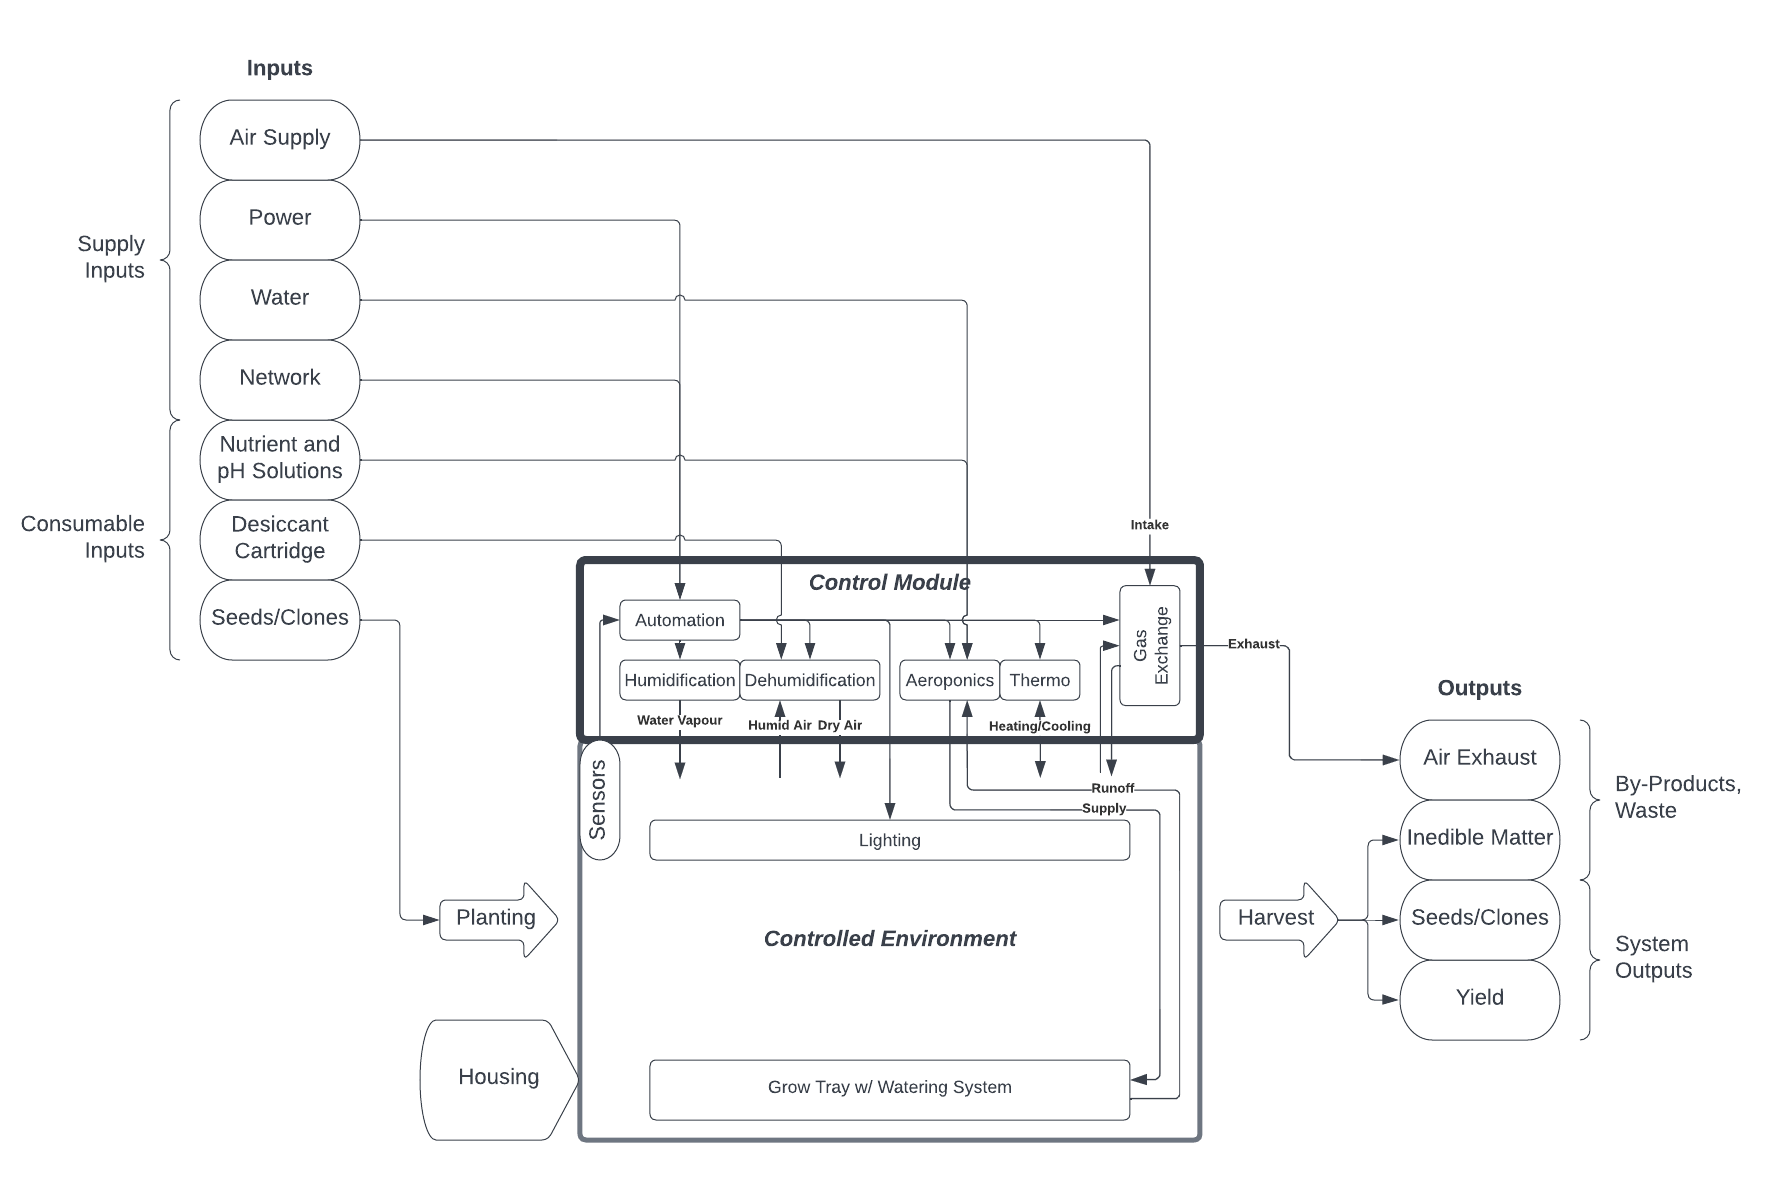
\includegraphics[width=\textwidth]{../assets/figures/system.png}}
    \caption{System overview.}
    \label{fig:system}
\end{figure}

\clearpage

\subsubsection{Hazard Analysis: Crew Contact (Harvesting, Cleaning, Maintenance)}

\begin{table}[!ht]
    \begin{tabularx}{\linewidth}{|ll|X|}
    \hline \multicolumn{2}{|l|}
        {\textbf{Source}}           & Crew contact with system during harvesting, cleaning, and maintenance  \\ \hline \multicolumn{2}{|l|}
        {\textbf{Identification}}   & Pathogens (bacteria, fungi, viruses) transferred from crew to system   \\ \hline \multicolumn{1}{|l|}{\multirow{3}{*}
        {\textbf{Evaluation}}}
        & \textit{Severity}         & Transfer of biological pathogens onto system surfaces has the potential to infect crops, posing a hazard to crew health during harvesting and ingestion. \\ \cline{2-3} \multicolumn{1}{|l|}{}
        & \textit{Likelihood}       & Fungi and viruses are of very low probability, as they cannot live on surfaces. Human gut bacteria (i.e. E. coli) is of low probability, as crew sanitation procedures are well-established. \\ \cline{2-3} \multicolumn{1}{|l|}{}
        & \textit{CCP?}             & The HACCP team determines that the risks of cross-contamination or infection are very low. Crew sanitation practices (especially prior to system interaction), practices that minimize system interaction, and sanitizing food outputs prior to consumption are adequate to control this potential hazard. \\ \hline
    \end{tabularx}
    \caption{Hazard analysis: pathogens transferred from crew to system.}
    \label{tab:hazardanalysis_systemcontact_1}
\end{table}

\begin{table}[!ht]
    \begin{tabularx}{\linewidth}{|ll|X|}
    \hline \multicolumn{2}{|l|}
        {\textbf{Source}}           & Crew contact with system during harvesting, cleaning, and maintenance \\ \hline \multicolumn{2}{|l|}
        {\textbf{Identification}}   & Pathogens (bacteria, fungi, viruses) transferred from system to crew \\ \hline \multicolumn{1}{|l|}{\multirow{3}{*}
        {\textbf{Evaluation}}}
        & \textit{Severity}         & Biological pathogens present in system materials have the potential to infect crew during interaction. \\ \cline{2-3} \multicolumn{1}{|l|}{}
        & \textit{Likelihood}       & All pathogens are of moderate probability, as they can be present in infected seeds (and thus food products at the time of ingestion). However, there are no known instances of plant-borne pathogens infecting humans. Bacteria can also be present on all surfaces. \\ \cline{2-3} \multicolumn{1}{|l|}{}
        & \textit{CCP?}             & The HACCP team determines that the risks of infection are low. However, for the sake of maximizing yield acceptability and consistency, care should be taken in seed sanitization. This, along with system sanitation practices (both pre-flight and during harvest) and practices that minimize system interaction, are adequate to control this potential hazard. \\ \hline
    \end{tabularx}
    \caption{Hazard analysis: pathogens transferred from system to crew.}
    \label{tab:hazardanalysis_systemcontact_2}
\end{table}

\clearpage

\begin{table}[!ht]
    \begin{tabularx}{\linewidth}{|ll|X|}
    \hline \multicolumn{2}{|l|}
        {\textbf{Source}}           & Crew contact with system during harvesting, cleaning, and maintenance \\ \hline \multicolumn{2}{|l|}
        {\textbf{Identification}}   & Chemical hazards to crew (i.e. heavy metals, process chemicals) introduced by system \\ \hline \multicolumn{1}{|l|}{\multirow{3}{*}
        {\textbf{Evaluation}}}
        & \textit{Severity}         & Heavy metals (i.e. lead) and chemicals introduced during manufacturing pose a threat to crew health, either during system interaction or food product ingestion. In addition, process chemicals (i.e. acidic/ basic solutions) can pose a hazard either through physical contact or accidental ingestion. \\ \cline{2-3} \multicolumn{1}{|l|}{}
        & \textit{Likelihood}       & Heavy metals are of low probability, but may be present in trace amounts in components (i.e. plumbing, electronics) and thus may come either in direct physical contact with crew(i.e. during maintenance) or be present in food products (i.e. uptake via water supply). \\ \cline{2-3} \multicolumn{1}{|l|}{}
        & \textit{CCP?}             & The HACCP team determines that the risks of heavy metal ingestion are low. All electronics, circuit boards, solder, plumbing fittings, are certified lead-free. All soldered surfaces are cleaned of flux residue. In addition, the aeroponic system is flushed of all process chemicals prior to crew interaction. Practices that include cleaning system surfaces after manufacturing, wearing gloves during handling and interaction, and cleaning food outputs of residue prior to consumption, are adequate to control this potential hazard. \\ \hline
    \end{tabularx}
    \caption{Hazard analysis: chemical hazards to system introduced by crew.}
    \label{tab:hazardanalysis_systemcontact_3}
\end{table}

\begin{table}[!ht]
    \begin{tabularx}{\linewidth}{|ll|X|}
    \hline \multicolumn{2}{|l|}
        {\textbf{Source}}           & Crew contact with system during harvesting, cleaning, and maintenance \\ \hline \multicolumn{2}{|l|}
        {\textbf{Identification}}   & Chemical hazards to system (i.e. disinfectants) introduced by crew \\ \hline \multicolumn{1}{|l|}{\multirow{3}{*}
        {\textbf{Evaluation}}}
        & \textit{Severity}         & Chemicals can remain on system surfaces, and may be present in food product, posing a hazard either through physical contact with surfaces or through ingestion. \\ \cline{2-3} \multicolumn{1}{|l|}{}
        & \textit{Likelihood}       & Disinfectants are of moderate probability. In addition, process chemicals used during maintenance (i.e. descaling agents for the aeroponics system) may be present on food product surfaces (i.e. root vegetables). \\ \cline{2-3} \multicolumn{1}{|l|}{}
        & \textit{CCP?}             & The HACCP team determines that the risks of chemical ingestion are low. Disinfectants are food-safe and dilute. In addition, the aeroponic system is flushed of all process chemicals prior to crew interaction. Practices that include wearing gloves during handling and interaction, wiping surfaces and food products with pure water prior to physical contact and ingestion, and practices that minimize system interaction are adequate to control this potential hazard. \\ \hline
    \end{tabularx}
    \caption{Hazard analysis: chemical hazards to crew introduced by system.}
    \label{tab:hazardanalysis_systemcontact_4}
\end{table}

\clearpage

\subsubsection{Hazard Analysis: Water Supply}
\begin{table}[!ht]
    \begin{tabularx}{\linewidth}{|ll|X|}
    \hline \multicolumn{2}{|l|}
        {\textbf{Source}}           & Water supply as a medium for accumulation and distribution of hazards \\ \hline \multicolumn{2}{|l|}
        {\textbf{Identification}}   & Chemical hazards (i.e. heavy metals, process chemicals) build up in water supply and transfer to produce and, in turn, crew  \\ \hline \multicolumn{1}{|l|}{\multirow{3}{*}
        {\textbf{Evaluation}}}
        & \textit{Severity}         & Heavy metals (i.e. lead) and chemicals introduced during manufacturing and process pose a threat to crew health when ingested via food product ingestion. In addition, buildup can compromise other systems (i.e. flow rate) and reduce resistance to other threats. \\ \cline{2-3} \multicolumn{1}{|l|}{}
        & \textit{Likelihood}       & Heavy metals are of low probability, but may be present in trace amounts in components (i.e. plumbing, electronics) and thus may be present in water supply for periods of time. However, regular flushing and cleansing of the supply will provide an upper bound on possible concentrations both in the supply and in any given produce. \\ \cline{2-3} \multicolumn{1}{|l|}{}
        & \textit{CCP?}             & The HACCP team determines that the risks of chemical accumulation are low. All electronics, circuit boards, solder, plumbing fittings, are certified lead-free. All soldered surfaces are cleaned of flux residue. In addition, the aeroponic system is flushed of all process chemicals prior to crew interaction. Practices that include cleaning system surfaces after manufacturing, wearing gloves during handling and interaction, and cleaning food outputs of residue prior to consumption, are adequate to control this potential hazard. \\ \hline
    \end{tabularx}
    \caption{Hazard analysis: chemical hazards accumulate in water system.}
    \label{tab:hazardanalysis_watersupply_1}
\end{table}

\begin{table}[!ht]
    \begin{tabularx}{\linewidth}{|ll|X|}
    \hline \multicolumn{2}{|l|}
        {\textbf{Source}}           & Water supply as a medium for accumulation and distribution of hazards \\ \hline \multicolumn{2}{|l|}
        {\textbf{Identification}}   & Bacteria present in water supply thrive, transfer to produce and, in turn, crew\\ \hline \multicolumn{1}{|l|}{\multirow{3}{*}
        {\textbf{Evaluation}}}
        & \textit{Severity}         & Bacteria in/on produce, surfaces, or suspended in mist can infect crew.  \\ \cline{2-3} \multicolumn{1}{|l|}{}
        & \textit{Likelihood}       & Probability of human-borne bacteria (i.e. \textit{E. coli}) is unlikely given stringent crew sanitation procedures. Other sources are infected seeds, however there are no known instances of plant-borne pathogens infecting humans. \\ \cline{2-3} \multicolumn{1}{|l|}{}
        & \textit{CCP?}             & The HACCP team determines that the risks of bacteria accumulation are low. Practices that include cleaning system surfaces after interaction, wearing gloves during handling, and flushing the water system regularly are adequate to control this potential hazard. \\ \hline
    \end{tabularx}
    \caption{Hazard analysis: bacteria grow in water system.}
    \label{tab:hazardanalysis_watersupply_2}
\end{table}

\clearpage
\subsubsection{Hazard Analysis: Nutrient Supply}
\begin{table}[!ht]
    \begin{tabularx}{\linewidth}{|ll|X|}
    \hline \multicolumn{2}{|l|}
        {\textbf{Source}}           & Nutrient Supply as a medium for accumulation and distribution of hazards \\ \hline \multicolumn{2}{|l|}
        {\textbf{Identification}}   & Bacteria in nutrient supply thrive, transfer to water and, in turn, crew  \\ \hline \multicolumn{1}{|l|}{\multirow{3}{*}
        {\textbf{Evaluation}}}
        & \textit{Severity}         & Bacteria from nutrient supply can be distributed throughout the system and infect crew. \\ \cline{2-3} \multicolumn{1}{|l|}{}
        & \textit{Likelihood}       & Nutrient supply is kept in pre-sealed packets of individual doses, meaning control on earth will eliminate introduction of threats via nutrient supply. Once in use, any bacteria will have come from the system, so presence in the nutrient supply is non-additive. \\ \cline{2-3} \multicolumn{1}{|l|}{}
        & \textit{CCP?}             & The HACCP team determines that the risks of biological threats in the nutrient supply are low. Given proper care in pre-flight steps and standard operating procedures when interacting with nutrient supply, enough practices are in place to control this hazard. \\ \hline
    \end{tabularx}
    \caption{Hazard analysis: bacteria grow in water system.}
    \label{tab:hazardanalysis_nutrientsupply_1}
\end{table}

\clearpage

\subsubsection{Hazard Analysis: Seeds}
\begin{table}[!ht]
    \begin{tabularx}{\linewidth}{|ll|X|}
    \hline \multicolumn{2}{|l|}
        {\textbf{Source}}           & Nutrient Supply as a medium for introduction of hazards \\ \hline \multicolumn{2}{|l|}
        {\textbf{Identification}}   & Pathogens (bacteria, fungi, viruses) present in seed supply are introduced to system  \\ \hline \multicolumn{1}{|l|}{\multirow{3}{*}
        {\textbf{Evaluation}}}
        & \textit{Severity}         & Minimal, there are no known occurences of plant-borne pathogens infecting humans.\\ \cline{2-3} \multicolumn{1}{|l|}{}
        & \textit{Likelihood}       & Moderate, however introduction of a pathogen will have occured pre-flight. But, they are sanitized and stored in isolated pouches which also minimize likelihood of bacteria on their surfaces.\\ \cline{2-3} \multicolumn{1}{|l|}{}
        & \textit{CCP?}             & The HACCP team determines that the risks of biological threats in the seed supply are low. Given proper care in pre-flight steps and standard operating procedures when planting seeds, enough practices are in place to control this minimally risky hazard. \\ \hline
    \end{tabularx}
    \caption{Hazard analysis: bacteria grow in water system.}
    \label{tab:hazardanalysis_nutrientsupply_1}
\end{table}


\subsection{Critical Points}

No critical points were identified in hazard analysis.
%assembly: only approved parts that have been checked for leaks, contamination, materials, air-tightness

%seeds: vetted and tested breed from an approved supplier, not opened until moment of planting, food safety steps followed while doing so (hand washing, gloves, masks, hairnet...)

%growth medium: tested for bacteria/pests, handled carefully before installation

%system inputs: filtered air, clean water, properly sourced nutrients, all tested by appropriate standards

%maintenance: plants properly isolated when non-food safe materials are present---i.e. if LED boards need to be swapped, if something needs to be greased, if something needs to be glued

%harvesting: all food safety guidelines to be followed - hand washing, gloves, masks, washing, etc.

%re-planting: checking for no old growth medium, sanitizing growth tray with food-safe sanitizer

% \subsubsection{Critical Point A}
% % Repeat for all control points

% \textbf{Hazard Description}
% % aka hazard analysis, discover CCPs

% \textbf{Critical Limits}
% % What is the safe range AND the failure conditions for the CCP

% \textbf{Monitoring Procedures}
% % How do we know the state of the CCP

% \textbf{Deviation Procedures}
% % aka corrective actions
% % How do we keep the CCP within range?

% \textbf{Associated Documents}
% record-keeping and documentation procedures

% TODO: Verification Procedures?

\subsection{Standard Test Record}
% TODO: What exactly is this?

% EXAMPLE

% Record for ingredients/materials for which critical limits have been established.
    % Supplier certification records documenting compliance of an ingredient/material with a critical limit.
    % Processor audit records verifying supplier compliance.
    % Storage records (e.g., time, temperature) for when ingredient/material storage is a CCP.

% Processing, storage and distribution records
    % Information that establishes the efficacy of a CCP to maintain product safety.
    % Data establishing the safe shelf life of the product; if age of product can affect safety.
    % Records indicating compliance with critical limits when packaging materials, labeling or sealing specifications are necessary for food safety.
    % Monitoring records.
    % Verification records.

% Deviation and corrective action records.

% Employee training records that are pertinent to CCPs and the HACCP plan.

% Documentation of the adequacy of the HACCP plan from a knowledgeable HACCP expert.

No critical points were identified in hazard analysis.

% \subsubsection{Purpose and Summary}

% \subsubsection{Safety and Quality}

% \subsubsection{Test Processes}

% \textbf{Preparation of Inputs}\\


% \textbf{Verification}\\


% \textbf{Setup, Maintenance, and Collection Protocols}\\


% \textbf{Storage}\\


% \textbf{Cleanup and Turnover}\\


% \subsubsection{Closeout}



\newpage

% References
\bibliographystyle{IEEEtran}
\bibliography{references}
\end{document}

\clearpage

\section{Hazard Analysis and Critical Control Point (HACCP) Plan}
% Specific focus on the safety of the system's processes and food outputs

% HACCP is a systematic approach to the identification, evaluation, and control of food safety hazards. A HACCP Plan is the written document which is based upon the principles of HACCP and which delineates the procedures to be followed.
% The Teams’ HACCP Plan should follow the principles and guidelines of a HACCP Plan as described by the U.S. National Advisory Committee on Microbiological Criteria for Foods (NACMCF) and the associated prerequisite programs (where applicable).
% The Basic HACCP Plan desired at this Progress Report stage (May 31 deadline) is only expected to be a starting point for the final Basic HACCP Plan expected to be a part of the final report (due in January 2023).

% Def'n of terms: https://www.fda.gov/food/hazard-analysis-critical-control-point-haccp/haccp-principles-application-guidelines#princ
% HACCP reference: https://spinoff.nasa.gov/moon-landing-food-safety?utm_source=TWITTER&utm_medium=KathyLueders&utm_campaign=NASASocial&linkId=141839394

\subsection{Food Production System Description}
% Incl. flowchart

% PeaPod uses automated control systems to generate desired environments. These are air thermoregulation, humidity control, LED lighting, and an aeroponics system. They are automated by an onboard computer and housed in a "control module" at the top of the unit. This lets power be "multiplied" for extended PeaPods by adding more control modules in a controller-follower topology.

% PeaPod is an automated plant growth environment, comprised of several control systems regulated by an automation and monitoring system within a modular, cubic housing. It can generate any desired environment while collecting data on plant growth and improving yields. Due to the wide range of actuation for each control system's environment parameter, and the extendable housing topology, the growth environment is adaptable to any plant or mission requirements. In addition, plant growth support platforms (with watering system) and lighting systems are built on modular "trays" mounted to the inside of the housing so the user can position plants and lights to accommodate any plant size.

% PeaPod's control systems are made of environmental controls (feedback loops with sensors) and plant inputs (set-states):
% \begin{itemize}
%     \item\textit{Lighting}: A wide spectrum of LEDs, from IR to UV, with a focus on Photosynthetically Active Radiation (PAR). Dimmable LED drivers enable precision spectrum and intensity control. Efficient, precise emission spectrum, low heat.
%     \item \textit{Aeroponics}: Reverse osmosis (RO) water is pressurized by a pump (with sensor for safety cutoff), brought to temperature, nutrient-dosed and pH-balanced by custom peristaltic pumps (allows for accurate dosing, and prevents backflow under pressure), and forced through nozzles to generate mist. Root zone air temperature is regulated in the same way as the leaf zone system. Exceptions include an aluminum water block (vs internal heat sink and fan) and a single temperature sensor after the block for PID feedback in a flowing system. Runoff water is recycled. Water-efficient (98\% less water use than farming), nutrient-efficient (60\% less use than farming), no pH/nutrient "feedback" loop or waste water (common in hydroponics), increased root oxygenation.
%     \item \textit{Leaf-Zone Thermoregulation}: Leaf zone air temperature is regulated by a thermoelectric heat pump. Fans blow air over heat sinks connected to either face of a Peltier tile to circulate air and dissipate heat. A Proportionate-Integral-Derivative (PID) control system is informed by temperature sensors, and controls the direction and magnitude of the heat transfer. Low complexity, high safety/reliability, easy to automate (bidirectional, precisely dimmable, PID tuning).
%     \item \textit{Humidity Regulation}: Leaf zone humidity is regulated by a dead-zone bang-bang control system informed by humidity sensors.
%     \begin{itemize}
%         \item \textit{Humidification}: RO water is supplied to a tank with a fine mesh piezoelectric disc. A controllable driver circuit oscillates the disk, producing water vapour. Easy to automate.
%         \item \textit{Dehumidification}: A dry silica gel bead cartridge is covered by servo-actuated "shutters" to control dehumidification. Fans draw humid air through a HEPA filter into the desiccant and back into the growth environment on demand. The beads change color to indicate water saturation. The crew is then notified to swap and "recharge" via evaporation in a standard oven.
%     \end{itemize}
%     \item \textit{Gas Composition Regulation and Exchange}: Oxygen and carbon dioxide levels are managed by gas exchange. Input and output ports allow fans to draw air into and out of the system. HEPA filters remove microbes and aerosols, and servo-actuated "shutters" prevent unintended exchange. Gas concentration sensors inform a bang-bang control system for port activation.
% \end{itemize}

\begin{figure}[h!]
    \centering
    \frame{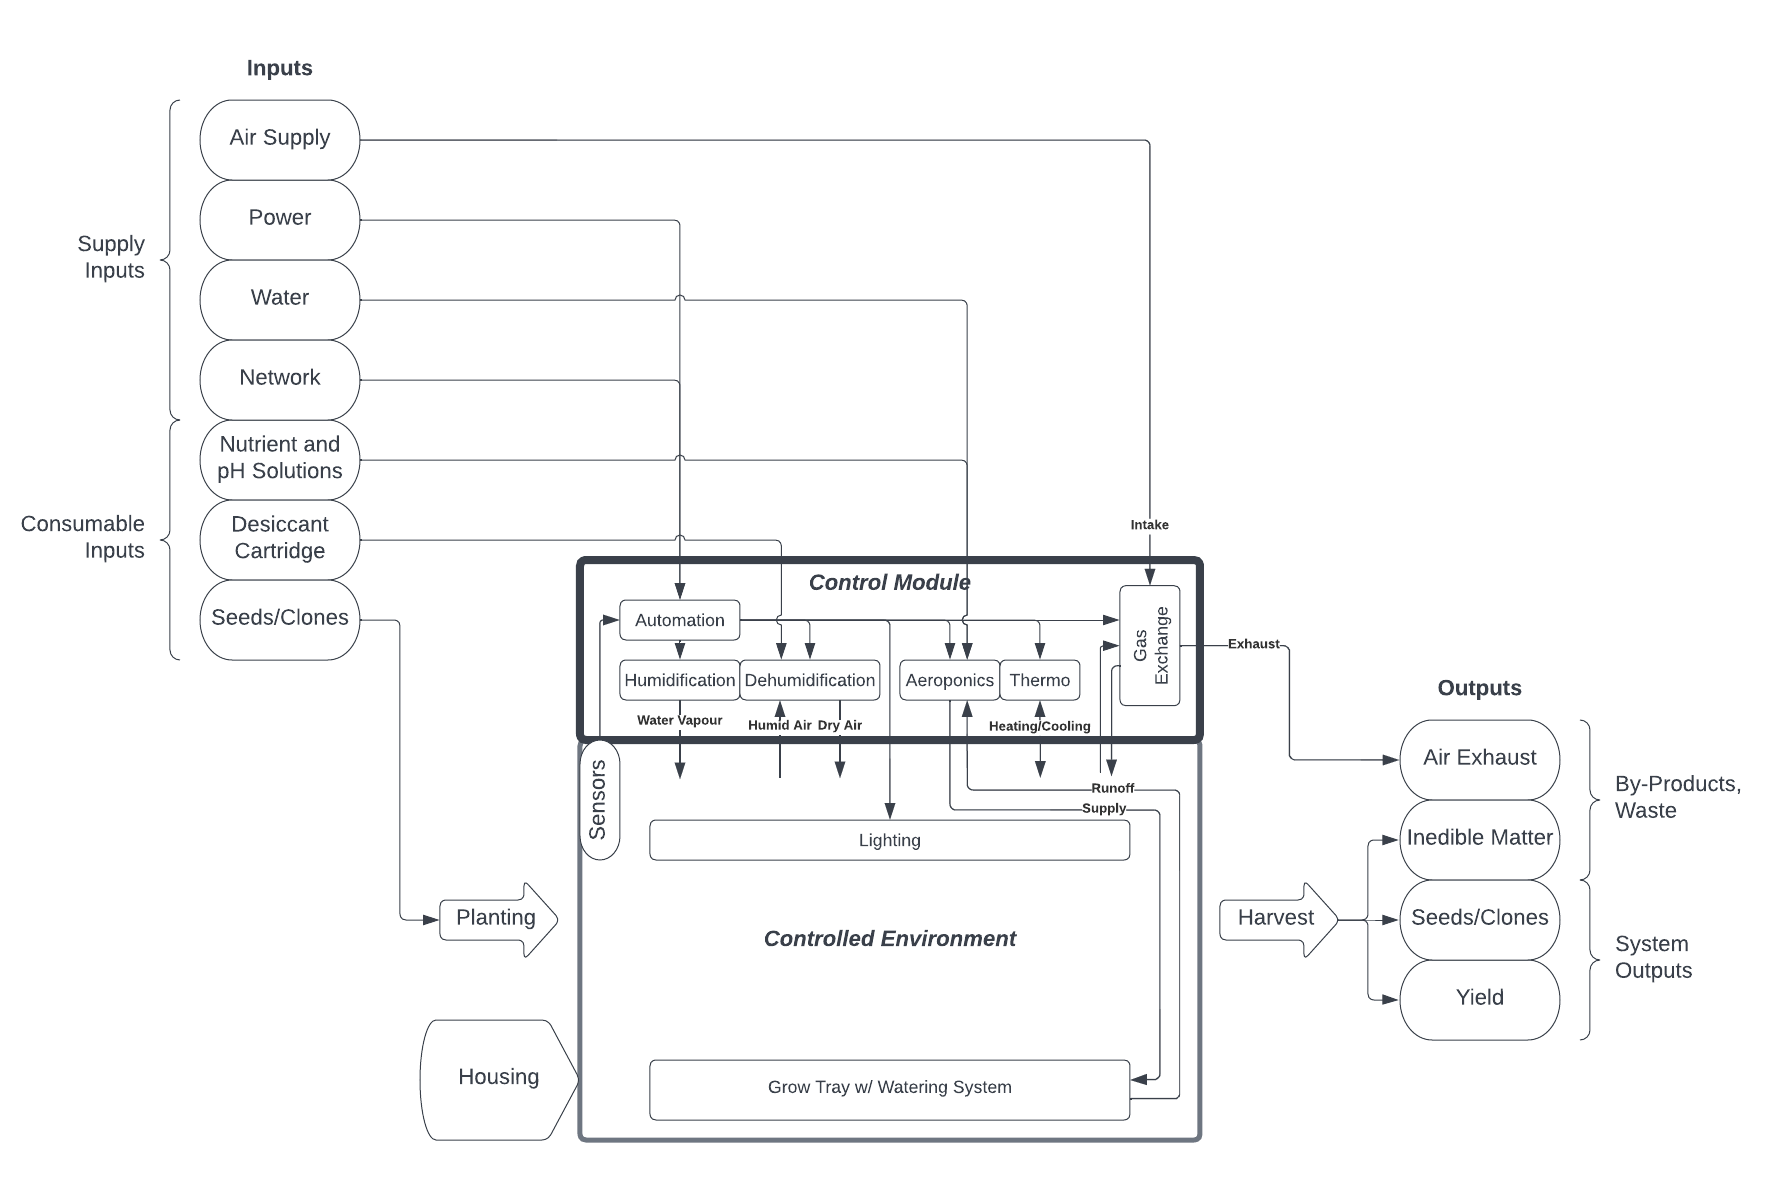
\includegraphics[width=\textwidth]{../assets/figures/system.png}}
    \caption{System overview.}
    \label{fig:system}
\end{figure}

\clearpage

\subsubsection{Hazard Analysis: Crew Contact (Harvesting, Cleaning, Maintenance)}

\begin{table}[!ht]
    \begin{tabularx}{\linewidth}{|ll|X|}
    \hline \multicolumn{2}{|l|}
        {\textbf{Source}}           & Crew contact with system during harvesting, cleaning, and maintenance  \\ \hline \multicolumn{2}{|l|}
        {\textbf{Identification}}   & Pathogens (bacteria, fungi, viruses) transferred from crew to system   \\ \hline \multicolumn{1}{|l|}{\multirow{3}{*}
        {\textbf{Evaluation}}}
        & \textit{Severity}         & Transfer of biological pathogens onto system surfaces has the potential to infect crops, posing a hazard to crew health during harvesting and ingestion. \\ \cline{2-3} \multicolumn{1}{|l|}{}
        & \textit{Likelihood}       & Fungi and viruses are of very low probability, as they cannot live on surfaces. Human gut bacteria (i.e. E. coli) is of low probability, as crew sanitation procedures are well-established. \\ \cline{2-3} \multicolumn{1}{|l|}{}
        & \textit{CCP?}             & The HACCP team determines that the risks of cross-contamination or infection are very low. Crew sanitation practices (especially prior to system interaction), practices that minimize system interaction, and sanitizing food outputs prior to consumption are adequate to control this potential hazard. \\ \hline
    \end{tabularx}
    \caption{Hazard analysis: pathogens transferred from crew to system.}
    \label{tab:hazardanalysis_systemcontact_1}
\end{table}

\begin{table}[!ht]
    \begin{tabularx}{\linewidth}{|ll|X|}
    \hline \multicolumn{2}{|l|}
        {\textbf{Source}}           & Crew contact with system during harvesting, cleaning, and maintenance \\ \hline \multicolumn{2}{|l|}
        {\textbf{Identification}}   & Pathogens (bacteria, fungi, viruses) transferred from system to crew \\ \hline \multicolumn{1}{|l|}{\multirow{3}{*}
        {\textbf{Evaluation}}}
        & \textit{Severity}         & Biological pathogens present in system materials have the potential to infect crew during interaction. \\ \cline{2-3} \multicolumn{1}{|l|}{}
        & \textit{Likelihood}       & All pathogens are of moderate probability, as they can be present in infected seeds (and thus food products at the time of ingestion). However, there are no known instances of plant-borne pathogens infecting humans. Bacteria can also be present on all surfaces. \\ \cline{2-3} \multicolumn{1}{|l|}{}
        & \textit{CCP?}             & The HACCP team determines that the risks of infection are low. However, for the sake of maximizing yield acceptability and consistency, care should be taken in seed sanitization. This, along with system sanitation practices (both pre-flight and during harvest) and practices that minimize system interaction, are adequate to control this potential hazard. \\ \hline
    \end{tabularx}
    \caption{Hazard analysis: pathogens transferred from system to crew.}
    \label{tab:hazardanalysis_systemcontact_2}
\end{table}

\clearpage

\begin{table}[!ht]
    \begin{tabularx}{\linewidth}{|ll|X|}
    \hline \multicolumn{2}{|l|}
        {\textbf{Source}}           & Crew contact with system during harvesting, cleaning, and maintenance \\ \hline \multicolumn{2}{|l|}
        {\textbf{Identification}}   & Chemical hazards to crew (i.e. heavy metals, process chemicals) introduced by system \\ \hline \multicolumn{1}{|l|}{\multirow{3}{*}
        {\textbf{Evaluation}}}
        & \textit{Severity}         & Heavy metals (i.e. lead) and chemicals introduced during manufacturing pose a threat to crew health, either during system interaction or food product ingestion. In addition, process chemicals (i.e. acidic/ basic solutions) can pose a hazard either through physical contact or accidental ingestion. \\ \cline{2-3} \multicolumn{1}{|l|}{}
        & \textit{Likelihood}       & Heavy metals are of low probability, but may be present in trace amounts in components (i.e. plumbing, electronics) and thus may come either in direct physical contact with crew(i.e. during maintenance) or be present in food products (i.e. uptake via water supply). \\ \cline{2-3} \multicolumn{1}{|l|}{}
        & \textit{CCP?}             & The HACCP team determines that the risks of heavy metal ingestion are low. All electronics, circuit boards, solder, plumbing fittings, are certified lead-free. All soldered surfaces are cleaned of flux residue. In addition, the aeroponic system is flushed of all process chemicals prior to crew interaction. Practices that include cleaning system surfaces after manufacturing, wearing gloves during handling and interaction, and cleaning food outputs of residue prior to consumption, are adequate to control this potential hazard. \\ \hline
    \end{tabularx}
    \caption{Hazard analysis: chemical hazards to system introduced by crew.}
    \label{tab:hazardanalysis_systemcontact_3}
\end{table}

\begin{table}[!ht]
    \begin{tabularx}{\linewidth}{|ll|X|}
    \hline \multicolumn{2}{|l|}
        {\textbf{Source}}           & Crew contact with system during harvesting, cleaning, and maintenance \\ \hline \multicolumn{2}{|l|}
        {\textbf{Identification}}   & Chemical hazards to system (i.e. disinfectants) introduced by crew \\ \hline \multicolumn{1}{|l|}{\multirow{3}{*}
        {\textbf{Evaluation}}}
        & \textit{Severity}         & Chemicals can remain on system surfaces, and may be present in food product, posing a hazard either through physical contact with surfaces or through ingestion. \\ \cline{2-3} \multicolumn{1}{|l|}{}
        & \textit{Likelihood}       & Disinfectants are of moderate probability. In addition, process chemicals used during maintenance (i.e. descaling agents for the aeroponics system) may be present on food product surfaces (i.e. root vegetables). \\ \cline{2-3} \multicolumn{1}{|l|}{}
        & \textit{CCP?}             & The HACCP team determines that the risks of chemical ingestion are low. Disinfectants are food-safe and dilute. In addition, the aeroponic system is flushed of all process chemicals prior to crew interaction. Practices that include wearing gloves during handling and interaction, wiping surfaces and food products with pure water prior to physical contact and ingestion, and practices that minimize system interaction are adequate to control this potential hazard. \\ \hline
    \end{tabularx}
    \caption{Hazard analysis: chemical hazards to crew introduced by system.}
    \label{tab:hazardanalysis_systemcontact_4}
\end{table}

\clearpage

\subsubsection{Hazard Analysis: Water Supply}
\begin{table}[!ht]
    \begin{tabularx}{\linewidth}{|ll|X|}
    \hline \multicolumn{2}{|l|}
        {\textbf{Source}}           & Water supply as a medium for accumulation and distribution of hazards \\ \hline \multicolumn{2}{|l|}
        {\textbf{Identification}}   & Chemical hazards (i.e. heavy metals, process chemicals) build up in water supply and transfer to produce and, in turn, crew  \\ \hline \multicolumn{1}{|l|}{\multirow{3}{*}
        {\textbf{Evaluation}}}
        & \textit{Severity}         & Heavy metals (i.e. lead) and chemicals introduced during manufacturing and process pose a threat to crew health when ingested via food product ingestion. In addition, buildup can compromise other systems (i.e. flow rate) and reduce resistance to other threats. \\ \cline{2-3} \multicolumn{1}{|l|}{}
        & \textit{Likelihood}       & Heavy metals are of low probability, but may be present in trace amounts in components (i.e. plumbing, electronics) and thus may be present in water supply for periods of time. However, regular flushing and cleansing of the supply will provide an upper bound on possible concentrations both in the supply and in any given produce. \\ \cline{2-3} \multicolumn{1}{|l|}{}
        & \textit{CCP?}             & The HACCP team determines that the risks of chemical accumulation are low. All electronics, circuit boards, solder, plumbing fittings, are certified lead-free. All soldered surfaces are cleaned of flux residue. In addition, the aeroponic system is flushed of all process chemicals prior to crew interaction. Practices that include cleaning system surfaces after manufacturing, wearing gloves during handling and interaction, and cleaning food outputs of residue prior to consumption, are adequate to control this potential hazard. \\ \hline
    \end{tabularx}
    \caption{Hazard analysis: chemical hazards accumulate in water system.}
    \label{tab:hazardanalysis_watersupply_1}
\end{table}

\begin{table}[!ht]
    \begin{tabularx}{\linewidth}{|ll|X|}
    \hline \multicolumn{2}{|l|}
        {\textbf{Source}}           & Water supply as a medium for accumulation and distribution of hazards \\ \hline \multicolumn{2}{|l|}
        {\textbf{Identification}}   & Bacteria present in water supply thrive, transfer to produce and, in turn, crew\\ \hline \multicolumn{1}{|l|}{\multirow{3}{*}
        {\textbf{Evaluation}}}
        & \textit{Severity}         & Bacteria in/on produce, surfaces, or suspended in mist can infect crew.  \\ \cline{2-3} \multicolumn{1}{|l|}{}
        & \textit{Likelihood}       & Probability of human-borne bacteria (i.e. \textit{E. coli}) is unlikely given stringent crew sanitation procedures. Other sources are infected seeds, however there are no known instances of plant-borne pathogens infecting humans. \\ \cline{2-3} \multicolumn{1}{|l|}{}
        & \textit{CCP?}             & The HACCP team determines that the risks of bacteria accumulation are low. Practices that include cleaning system surfaces after interaction, wearing gloves during handling, and flushing the water system regularly are adequate to control this potential hazard. \\ \hline
    \end{tabularx}
    \caption{Hazard analysis: bacteria grow in water system.}
    \label{tab:hazardanalysis_watersupply_2}
\end{table}

\clearpage
\subsubsection{Hazard Analysis: Nutrient Supply}
\begin{table}[!ht]
    \begin{tabularx}{\linewidth}{|ll|X|}
    \hline \multicolumn{2}{|l|}
        {\textbf{Source}}           & Nutrient Supply as a medium for accumulation and distribution of hazards \\ \hline \multicolumn{2}{|l|}
        {\textbf{Identification}}   & Bacteria in nutrient supply thrive, transfer to water and, in turn, crew  \\ \hline \multicolumn{1}{|l|}{\multirow{3}{*}
        {\textbf{Evaluation}}}
        & \textit{Severity}         & Bacteria from nutrient supply can be distributed throughout the system and infect crew. \\ \cline{2-3} \multicolumn{1}{|l|}{}
        & \textit{Likelihood}       & Nutrient supply is kept in pre-sealed packets of individual doses, meaning control on earth will eliminate introduction of threats via nutrient supply. Once in use, any bacteria will have come from the system, so presence in the nutrient supply is non-additive. \\ \cline{2-3} \multicolumn{1}{|l|}{}
        & \textit{CCP?}             & The HACCP team determines that the risks of biological threats in the nutrient supply are low. Given proper care in pre-flight steps and standard operating procedures when interacting with nutrient supply, enough practices are in place to control this hazard. \\ \hline
    \end{tabularx}
    \caption{Hazard analysis: bacteria grow in water system.}
    \label{tab:hazardanalysis_nutrientsupply_1}
\end{table}

\clearpage

\subsubsection{Hazard Analysis: Seeds}
\begin{table}[!ht]
    \begin{tabularx}{\linewidth}{|ll|X|}
    \hline \multicolumn{2}{|l|}
        {\textbf{Source}}           & Nutrient Supply as a medium for introduction of hazards \\ \hline \multicolumn{2}{|l|}
        {\textbf{Identification}}   & Pathogens (bacteria, fungi, viruses) present in seed supply are introduced to system  \\ \hline \multicolumn{1}{|l|}{\multirow{3}{*}
        {\textbf{Evaluation}}}
        & \textit{Severity}         & Minimal, there are no known occurences of plant-borne pathogens infecting humans.\\ \cline{2-3} \multicolumn{1}{|l|}{}
        & \textit{Likelihood}       & Moderate, however introduction of a pathogen will have occured pre-flight. But, they are sanitized and stored in isolated pouches which also minimize likelihood of bacteria on their surfaces.\\ \cline{2-3} \multicolumn{1}{|l|}{}
        & \textit{CCP?}             & The HACCP team determines that the risks of biological threats in the seed supply are low. Given proper care in pre-flight steps and standard operating procedures when planting seeds, enough practices are in place to control this minimally risky hazard. \\ \hline
    \end{tabularx}
    \caption{Hazard analysis: bacteria grow in water system.}
    \label{tab:hazardanalysis_nutrientsupply_1}
\end{table}


\subsection{Critical Points}

No critical points were identified in hazard analysis.
%assembly: only approved parts that have been checked for leaks, contamination, materials, air-tightness

%seeds: vetted and tested breed from an approved supplier, not opened until moment of planting, food safety steps followed while doing so (hand washing, gloves, masks, hairnet...)

%growth medium: tested for bacteria/pests, handled carefully before installation

%system inputs: filtered air, clean water, properly sourced nutrients, all tested by appropriate standards

%maintenance: plants properly isolated when non-food safe materials are present---i.e. if LED boards need to be swapped, if something needs to be greased, if something needs to be glued

%harvesting: all food safety guidelines to be followed - hand washing, gloves, masks, washing, etc.

%re-planting: checking for no old growth medium, sanitizing growth tray with food-safe sanitizer

% \subsubsection{Critical Point A}
% % Repeat for all control points

% \textbf{Hazard Description}
% % aka hazard analysis, discover CCPs

% \textbf{Critical Limits}
% % What is the safe range AND the failure conditions for the CCP

% \textbf{Monitoring Procedures}
% % How do we know the state of the CCP

% \textbf{Deviation Procedures}
% % aka corrective actions
% % How do we keep the CCP within range?

% \textbf{Associated Documents}
% record-keeping and documentation procedures

% TODO: Verification Procedures?

\subsection{Standard Test Record}
% TODO: What exactly is this?

% EXAMPLE

% Record for ingredients/materials for which critical limits have been established.
    % Supplier certification records documenting compliance of an ingredient/material with a critical limit.
    % Processor audit records verifying supplier compliance.
    % Storage records (e.g., time, temperature) for when ingredient/material storage is a CCP.

% Processing, storage and distribution records
    % Information that establishes the efficacy of a CCP to maintain product safety.
    % Data establishing the safe shelf life of the product; if age of product can affect safety.
    % Records indicating compliance with critical limits when packaging materials, labeling or sealing specifications are necessary for food safety.
    % Monitoring records.
    % Verification records.

% Deviation and corrective action records.

% Employee training records that are pertinent to CCPs and the HACCP plan.

% Documentation of the adequacy of the HACCP plan from a knowledgeable HACCP expert.

No critical points were identified in hazard analysis.

% \subsubsection{Purpose and Summary}

% \subsubsection{Safety and Quality}

% \subsubsection{Test Processes}

% \textbf{Preparation of Inputs}\\


% \textbf{Verification}\\


% \textbf{Setup, Maintenance, and Collection Protocols}\\


% \textbf{Storage}\\


% \textbf{Cleanup and Turnover}\\


% \subsubsection{Closeout}



\clearpage

\section{Feedback}
% Is there any feedback you would like to share with the Challenge Team? Do you have specific requests for topics, experts or information you would like to see discussed in the Phase 2 workshops?

No feedback is provided.

% Maximum 5000 characters

\clearpage

% References
\bibliographystyle{IEEEtran}
\bibliography{references}
\end{document}